\chapter{Simple Modules}
\label{cha:simple-modules}

The activities of simple\index{module!simple} modules are implemented by the user.
The algorithms are programmed in C++, using the {\opp} class
library. The following sections contain a short introduction
to discrete event simulation in general, how its concepts are
implemented in {\opp}, and gives an overview and practical advice
on how to design and code simple\index{module!simple} modules.




\section{Simulation concepts}

This section contains a very brief introduction into how Discrete
Event Simulation (DES) works, in order to introduce terms we'll use
when explaining {\opp} concepts\index{simulation!concepts} and
implementation. If you're familiar with DES\index{DES}, you can skip
the next few sections.




\subsection{Discrete Event Simulation}

A \textit{Discrete Event System} is a system where state changes
(events\index{events}) happen at discrete points of time, and events take zero time
to happen. It is assumed that nothing (i.e. nothing interesting)
happens between two consecutive events, that is, no state change takes
place in the system between the events (in contrast to
\textit{continuous} systems where state changes are continuous). Those
systems that can be viewed as Discrete Event Systems can be modeled
using Discrete Event Simulation\index{discrete event simulation}.
(Continuous systems are modelled using differential equations and
suchlike.)

For example, computer networks are usually viewed as discrete
event systems. Some of the events are:

\begin{itemize}
  \item{start of a packet transmission}
  \item{end of a packet transmission}
  \item{expiry of a retransmission timeout}
\end{itemize}


This implies that between two events such as \textit{start of a packet
transmission} and \textit{end of a packet transmission}, nothing
interesting happens. That is, the packet's state remains \textit{being
transmitted}. Note that the definition of ``interesting'' events and states always
depends on the intent and purposes of the person doing the modeling.
If we were interested in the transmission of individual bits, we would
have included something like \textit{start of bit transmission} and
\textit{end of bit transmission} among our events.


The time when events occur is often called \textit{event timestamp}
\index{event timestamp}; with {\opp} we'll say
\textit{arrival time}\index{arrival time} (because in the class
library, the word ``timestamp'' is reserved for a user-settable
attribute in the event class). Time within the model is often called
\textit{simulation time}\index{simulation time}, \textit{model time}
\index{model!time} or \textit{virtual time}\index{virtual time}
as opposed to real time\index{real time} or CPU time\index{CPU time}
or which refers to how long the simulation program has been running or
how much CPU time it has consumed.



\subsection{The event loop}

Discrete event simulations maintain the set of future
events\index{future events} in a data structure often called
FES\index{FES} (Future Event Set) or FEL\index{FEL} (Future Event List).
Such simulators usually work according to the following pseudocode:

\begin{Verbatim}[commandchars=\\\{\}]
\textit{initialize -- this includes building the model and}
              \textit{inserting initial events to FES}

\textit{while (FES not empty and simulation not yet complete)}
\textit{\{}
    \textit{retrieve first event from FES}
    \textit{t:= timestamp of this event}
    \textbf{\textit{process event}}
    \textit{(processing may insert new events in  FES or delete existing ones)}
\textit{\}}
\textit{finish simulation (write statistical results, etc.)}
\end{Verbatim}


The first, initialization step usually builds the data structures
representing the simulation model, calls any user-defined
initialization code, and inserts initial events\index{initial events}
into the FES to ensure that the simulation can start. Initialization
strategy can be quite different from one simulator to another.


The subsequent loop consumes events from the FES and processes
them. Events are processed in strict timestamp order in order
to maintain causality, that is, to ensure that no event may have
an effect on earlier events.

Processing an event involves calls to user-supplied code. For example,
using the computer network simulation example, processing a ``timeout
expired'' event may consist of re-sending a copy of the network
packet, updating the retry count, scheduling another ``timeout''
event, and so on. The user code may also remove events from the FES\index{FES},
for example when cancelling timeouts.

Simulation stops when there are no more events left (this happens
rarely in practice), or when it isn't necessary for the simulation
to run further because the model time or the CPU time has reached
a given limit, or because the statistics have reached the desired
accuracy. At this time, before the program exits, the simulation
programmer will typically want to record statistics into output
files.



\subsection{Simple modules in {\opp}}

In {\opp}, events occur inside simple modules\index{module!simple}.
Simple modules encapsulate C++ code that generate and react to events,
in other words, implement the behaviour of the model.

The user creates simple module types by subclassing the \cclass{cSimpleModule}
class, which is part of the {\opp} class library.
\cclass{cSimpleModule}, just as \cclass{cCompoundModule}, is derived
from a common base class, \cclass{cModule}.

\cclass{cSimpleModule}, although stuffed with simulation-related
functionality, doesn't do anything useful by itself -- you have
to redefine some virtual member functions to make it do useful work.


These member functions are the following:
\begin{itemize}
  \item{void \fname{initialize()}}
  \item{void \fname{activity()}}
  \item{void \fname[handleMessage()]{handleMessage(cMessage *msg)}}
  \item{void \fname{finish()}}
\end{itemize}

In the initialization step, {\opp} builds the network: it creates the
necessary simple\index{module!simple} and compound modules and
connects them according to the NED definitions. {\opp} also calls the
\fname{initialize()} functions of all modules.

The \fname{activity()} and \fname{handleMessage()} functions are
called during event processing. This means that the user will
implement the model's behavior in these functions.
\fname{activity()} and \fname{handleMessage()} implement
different event processing strategies\index{event processing
  strategies}: for each simple\index{module!simple} module, the user
has to redefine exactly one of these functions. \fname{activity()} is
a coroutine-based\index{coroutine} solution which implements the
process interaction approach (coroutines are non-pre\-emp\-tive
[cooperative] threads). \fname{handleMessage()} is a method that is called
by the simulation kernel when the module receives a message.
Modules written with \fname{activity()} and \fname{handleMessage()}
can be freely mixed within a simulation model.

The \fname{finish()} functions are called when the simulation
terminates successfully. The most typical use of \fname{finish()}
is the recording of statistics collected during simulation.

All these functions will be discussed later in detail.



\subsection{Events in {\opp}}

{\opp} uses messages\index{message} to represent
events\index{events}. Each event is represented by an instance of the
\cclass{cMessage} class or one its subclasses; there is no separate
event class. Messages are sent from one module to another -- this
means that the place where the ``event will occur'' is the
\textit{message's destination module}, and the model time when the
event occurs is the \textit{arrival time}\index{arrival time} of the
message. Events like ``timeout expired'' are implemented with the
module sending a message to itself.

Simulation time in {\opp} is stored in the C++ type
\fvar{simtime\_t}, which is a typedef for \fvar{double}.

Events are consumed from the FES\index{FES} in arrival time order, to
maintain causality. More precisely, given two messages, the following
rules apply:
\begin{enumerate}
\item{the message with \textbf{earlier arrival time} is executed
    first.  If arrival times are equal,}
\item{the one with \textbf{smaller priority value} is executed first.
    If priorities are the same,}
\item{the one \textbf{scheduled or sent earlier} is executed first.}
\end{enumerate}

\textit{Priority}\index{message!priority} is a user-assigned integer
attribute of messages.

Storing simulation time in doubles may sometimes cause inconveniences.
Due to finite machine precision, two doubles calculated in two
different ways do not always compare equal even if they mathematically
should be. For example, addition is not an associative operation
when it comes to floating point calculations: $(x+y)+z != x+(y+z)$!
  \footnote{see also \textit{``What Every Computer Scientist Should
  Know About Floating-Point Arithmetic''} by David Goldberg, 1991}
This means that if you want to explicitly rely on the
arrival times of two events being the same, you should take care that
they are calculated in exactly the same way.
Another possible approach is to avoid equal arrival times,
for example by adding/subtracting small values to schedule times to
ensure specific execution order
(\textit{inorder\_epsilon}\index{inorder\_epsilon}).

One may suggest introducing a small \textit{simtime\_precision} parameter in
the simulation kernel that would force $t_{1}$ and $t_{2}$ to be regarded
equal if they are ``very close'' (if they differ
less than \textit{simtime\_precision}). However, in addition to the problem
determining the correct value for \textit{simtime\_precision},
this approach is likely to cause confusion in many cases.



\subsection{FES implementation}

The implementation of the FES\index{FES} is a crucial factor in the
performance of a discrete event simulator. In {\opp}, the FES is
implemented with \textit{binary heap}\index{binary heap}, the most
widely used data structure for this purpose. Heap is also the best
algorithm we know, although exotic data structures like
\textit{skiplist}\index{skiplist} may perform better than heap in some
cases. In case you're interested, the FES implementation is in the
\cclass{cMessageHeap} class, but as a simulation programmer you won't
ever need to care about it.


\section{Defining simple module types}

\subsection{Overview}

The C++ implementation of a simple\index{module!simple} module consists of:
\begin{itemize}
\item{declaration of the module class: your class subclassed from \cclass{cSimpleModule}
(either directly or indirectly)}
\item{a module type registration (\fmac{Define\_Module()} or
    \fmac{Define\_Module\_Like()} macro)}
\item{implementation of the module class}
\end{itemize}


For example, the C++ source for a Sliding Window Protocol implementation
might look like this:

\begin{verbatim}
// file: swp.cc
#include <omnetpp.h>

// module class declaration:
class SlidingWindow : public cSimpleModule
{
    Module_Class_Members(SlidingWindow,cSimpleModule,8192)
    virtual void activity();
};

// module type registration:
Define_Module( SlidingWindow );

// implementation of the module class:
void SlidingWindow::activity()
{
  int windowSize = par("windowSize");
...
}
\end{verbatim}

In order to be able to refer to this simple\index{module!simple} module type in NED
files, we should have an associated NED declaration which might
look like this:


\begin{Verbatim}[commandchars=\\\{\}]
// file: swp.ned
\textbf{simple} SlidingWindow
    \textbf{parameters}:
        windowSize: \textbf{numeric const};
    \textbf{gates}:
        \textbf{in:} fromNet, fromUser;
        \textbf{out:} toNet, toUser;
\textbf{endsimple}
\end{Verbatim}




\subsection{The module declaration}
\index{module!declaration}

The module declaration
\begin{itemize}
\item{announces that you're going to use the class as a
    simple module type}
\item{associates the module class with an interface declared in NED}
\end{itemize}

\textbf{Forms of module declaration}


Module declarations can take two forms:

\begin{Verbatim}[commandchars=\\\{\}]
Define_Module(\textit{classname});
Define_Module_Like(\textit{classname}, \textit{neddeclname});
\end{Verbatim}

The first form associates the class (subclassed from
\cclass{cSimpleModule}) with the NED simple
module declaration of the same name. For example, the

\begin{verbatim}
Define_Module(SlidingWindow);
\end{verbatim}

line would ensure that when you create an instance of SlidingWindow in
your NED files, the module has the parameters and gates given in the
simple SlidingWindow NED declaration, and the implementation will be
an instance of the SlidingWindow C++ class.


The second form associates the class with a NED
simple module declaration of a different name.
You can use this form when you have several modules which share the
same interface. This feature will be discussed in detail in the next
section.


\textbf{Header files}


Module declarations should not be put into header files\index{header
  files}, because they are macros expanding to lines for which the
compiler generates code.


\textbf{Compound modules}

All module types (including compound\index{module!compound} modules)
need to have module declarations\index{module!declaration}. For all
compound modules, the NEDC compiler generates the
\fmac[Define\_Module()]{Define\_Module(..)} lines automatically.
However, it is your responsibility to put Define\_Module(..) lines into
one of the C++ sources for all your simple module types.


\textbf{Implementation}


Unless you are dying to learn about the dirty internals, you may just
as well skip this section. But if you're interested, here it is:
\fmac{Define\_Module()} (and also \fmac{Define\_Module\_Like()}) is a
macro which expands to a function definition plus the definition of a
global object, something like this ugly code (luckily, you won't ever
need to be interested in it):

\begin{Verbatim}[commandchars=\\\{\}]
static cModule *\textit{MyClass}__create(const char *name, cModule *parentmod)
{
    return (cModule *) new \textit{MyClass}(name, parentmod);
}

cModuleType \textit{MyClass}__type("\textit{MyClass}","\textit{MyClass}",
 (ModuleCreateFunc)\textit{MyClass}__create);
\end{Verbatim}


The \cclass{cModuleType} object can act as a factory: it is able to
create an instance of the given module type. This, together with the
fact that all \cclass{cModuleType} objects are available in a single
linked list, allows {\opp} to instantiate module types given only
their class names as strings, without having to include the class
declaration into any other C++ source.


The global object also stores the name of the NED
interface\index{ned!interface} associated with the module class. The
interface description object\index{interface description object}
(another object, generated by nedc) is looked up automatically at
network construction time. Whenever a module of the given type is
created, it will automatically have the parameters and gates specified
in the associated interface description.



\subsection{Several modules, single NED interface}

To support submodule types defined as parameters in
NED files (see section \ref{sec:ch-ned-lang:like}),
you can reuse an existing NED simple module definition
for several simple module types.

Suppose you have three different C++ module classes (\ttt{TokenRingMAC},
\ttt{EthernetMAC}, \ttt{FDDIMAC}) which have identical gates and parameters.
Then you can create a single NED declaration, \ttt{GenericMAC} for them
and write the following module declarations in the C++ code:

\begin{verbatim}
Define_Module_Like(TokenRingMAC, GenericMAC);
Define_Module_Like(EthernetMAC, GenericMAC);
Define_Module_Like(FDDIMAC, GenericMAC);
\end{verbatim}

You won't be able to directly refer to the \ttt{TokenRingMAC},
\ttt{EthernetMAC}, \ttt{FDDIMAC} module types in your NED files,
because NED doesn't know about them (their names don't appear
in any NED file you could import), but you can use them wherever
a submodule type was defined as a parameter to the compound module:

\begin{verbatim}
module Host
    parameters:
        macType: string;
    submodules:
        mac: macType like GenericMAC;
                // if macType=="EthernetMAC" --> OK!
     ...
endmodule
\end{verbatim}

\begin{sloppypar}
The \ttt{macType} parameter should take the value \texttt{"TokenRingMAC"},
\texttt{"EthernetMAC"} or \texttt{"FDDIMAC"}, and a submodule of the appropriate
type will be created. The value for the parameter can even be given in
the ini file. This gives you a powerful tool to customize simulation
models (see also \textit{Topology templates}, Section
\ref{sec:ch-ned-lang:topology-templates}).
\end{sloppypar}




\subsection{The class declaration}

As mentioned before, simple\index{module!simple} module classes have
to be derived from \cclass{cSimpleModule} (either directly or
indirectly). In addition to overwriting some of the previously
mentioned four member functions (\fname{initialize()},
\fname{activity()}, \fname{handleMessage()},\fname{finish()}), you
have to write a constructor\index{module!constructor} and some more
functions. Some of this task can be automated, so when writing the C++
class declaration, you have two choices:
\begin{enumerate}
\item{either use a macro which expands to the ``stock'' version of the
    functions}
\item{or write them yourself.}
\end{enumerate}

\textbf{Using macro to declare the constructor}

If you choose the first solution, you use the
\fmac{Module\_Class\_Members()} macro:

\begin{Verbatim}[commandchars=\\\{\}]
Module_Class_Members(\textit{classname}, \textit{baseclass}, \textit{stacksize});
\end{Verbatim}

The first two arguments are obvious (\textit{baseclass} is usually \cclass{cSimpleModule}),
but \textit{stacksize} needs some explanation. If you use \fname{activity()},
the module code runs as a coroutine\index{coroutine}, so it will need a separate
stack. (This will be discussed in detail later.)


As an example, the class declaration

\begin{verbatim}
class SlidingWindow : public cSimpleModule
{
    Module_Class_Members(SlidingWindow,cSimpleModule,8192)
    ...
};
\end{verbatim}

expands to something like this:

\begin{verbatim}
class SlidingWindow : public cSimpleModule
{
  public:
    SlidingWindow(const char *name, cModule *parentmodule,
        unsigned stacksize = 8192) :
        cSimpleModule(name, parentmodule, stacksize) {}
    ...
};
\end{verbatim}

\textbf{Expanded form of the constructor}

If you have data members in the class that you want to initialize in the
constructor, you cannot use the \ttt{Module_Class_Members()} macro.
Then you have to write the constructor yourself.

The constructor\index{module!constructor} should take the following
arguments (which you also have to pass further to the base class):

\begin{itemize}
  \item{\ttt{const char *name}, which is the name of the module}
  \item{\ttt{cModule *parentmodule}, pointer to the parent module}
  \item{\ttt{unsigned stacksize=\textit{stacksize}}, the coroutine stack size}
\end{itemize}

You should not change the number or types of the arguments taken
by the constructor, because it will be called by {\opp}-generated
code.

An example:

\begin{verbatim}
class TokenRingMAC : public cSimpleModule
{
  public:
    cQueue queue; // a data member
    TokenRingMAC(const char *name, cModule *parentmodule,
                 unsigned stacksize = 8192);
    ...
};

TokenRingMAC(const char *name, cModule *parentmodule,
    unsigned stacksize) :
    cSimpleModule(name, parentmodule, stacksize), queue("queue")
{
  // initialize data members
}
\end{verbatim}


\textbf{Stack size decides between activity() and handleMessage()}

\begin{itemize}
\item{if the specified stack size is zero, \fname{handleMessage()} will be used;}
\item{if it is greater than zero, \fname{activity()} will be used.}
\end{itemize}

If you make a mistake (e.g. you forget to set zero stack size
\index{zero stack size} for a \fname{handleMessage()}
simple module): the default versions of the
functions issue error messages telling you what is the problem.





\subsection{Decomposing activity()/handleMessage() and inheritance}

It is usually a good idea to decompose a \fname{activity()} or
\fname{handleMessage()} function when it grows too large. ``Too
large'' is a matter of taste of course, but you should definitely
consider splitting up the function if it is more that a few screens
(say 50-100 lines) long. This will have a couple of advantages:
\begin{itemize}
\item{will help future readers of the code understand your program;}
\item{will help \textit{you} understand what it is you're really programming
and bring some structure into it;}
\item{will enable you to customize the class by inheriting from it and
    overwriting member functions}
\end{itemize}

If you have variables which you want to access from all member
functions (typically state variables are like that), you'll need to
add those variables to the class as data members\index{class data
  members}.

Let's see an example:

\begin{verbatim}
class TransportProtocol : public cSimpleModule
{
  public:
    Module_Class_Members(TransportProtocol, cSimpleModule, 8192)
    int windowSize;
    int n_s; // N(s)
    int n_r; // N(r)
    cOutVector eedVector;
    cStdDev eedStats;
    //...

    virtual void activity();
    virtual void recalculateTimeout();
    virtual void insertPacketIntoBuffer(cMessage *packet);
    virtual void resendPacket(cMessage *packet);
    //...
};

Define_Module( TransportProtocol );

void TransportProtocol::activity()
{
    windowSize = par("windowSize");
    n_s = n_r = 0;
    eedVector.setName("End-to-End Delay");
    eedStats.setName("eedStats");
    //...
}

//...
\end{verbatim}

\begin{sloppypar}
  Note that you may have to use the expanded form of the
  constructor\index{module!constructor} (instead of
  \fmac{Module\_Class\_Members()}) to pass arguments to the constructors
  of member objects like eedVector and eedStats. But most often you
  don't need to go as far as that; for example, you can set parameters
  later from \fname{activity()}, as shown in the example above.
\end{sloppypar}

To implement another variant of the Transport Protocol which uses a
different timeout scheme, you could simply subclass TransportProtocol:

\begin{verbatim}
class AdvancedTransportProtocol : public TransportProtocol
{
  public:
    Module_Class_Members(AdvancedTransportProtocol, TransportProtocol,
                      8192)
    virtual void recalculateTimeout();
};

Define_Module( AdvancedTransportProtocol );

void AdvancedTransportProtocol::recalculateTimeout()
{
    //...
}
\end{verbatim}




\section{Adding functionality to cSimpleModule}

This section discusses \cclass{cSimpleModule}'s four previously
mentioned member functions, intended to be redefined by the user:
\fname{initialize()}, \fname{activity()}, \fname{handleMessage()} and
\fname{finish()}.


\subsection{activity()}

\textbf{Process-style description}

With \fname{activity()}, you can code the simple
module much like you would code an operating system process or a
thread. You can wait for an incoming message (event) at any point of
the code, you can suspend the execution for some time (model time!),
etc. When the \fname{activity()} function exits, the module is
terminated.  (The simulation can continue if there are other modules
which can run.)


The most important functions you can use in \fname{activity()} are
(they will be discussed in detail later):
\begin{itemize}
\item{\fname[receive()]{receive..()} family of functions -- to receive messages (events)}
\item{\fname{wait()} -- to suspend execution\index{suspend execution}
    for some time (model time)}
\item{\fname{send()} family of functions -- to send messages to other
    modules}
\item{\fname{scheduleAt()} -- to schedule an event (the module ``sends
    a message to itself'')}
\item{\fname{cancelEvent()} -- to delete an event scheduled with
    scheduleAt()}
\item{\fname{end()} -- to finish execution of this module (same as
    exiting the \fname{activity()} function)}
\end{itemize}

The \fname{activity()} function normally contains an infinite loop,
with at least a \fname{wait()} or \fname{receive()} call in its body.



\textbf{Application area}


One area where the process-style description\index{process-style
  description} is especially convenient is when the process has many
states but transitions are very limited, ie. from any state the
process can only go to one or two other states.  For example, this is
the case when programming a network application which uses a single
network connection.  The pseudocode of the application which talks to
a transport layer protocol might look like this:

\begin{Verbatim}[commandchars=\\\{\}]
\textit{activity()}
\{
    while(true)
    \{
        open connection by sending OPEN command to transport layer
        receive reply from transport layer
        if (open not successful)
        \{
            wait(some time)
            continue // loop back to while()
        \}

        while(there's more to do)
        \{
            send data on network connection
            if (connection broken)
            \{
                continue outer loop // loop back to outer while()
            \}
            wait(some time)
            receive data on network connection
            if (connection broken)
            \{
                continue outer loop // loop back to outer while()
            \}
            wait(some time)
        \}
        close connection by sending CLOSE command to transport layer
        if (close not successful)
        \{
            // handle error
        \}
        wait(some time)
    \}
\}
\end{Verbatim}



If you want to handle several connections simultaneously, you may
dynamically create as instances of the simple
module above as needed. Dynamic module creation will be discussed
later.


\textbf{Activity() is run as a coroutine}


\fname[activity()]{Activity()} is run in a coroutine\index{coroutine}.
Coroutines are a sort of threads\index{threads} which are scheduled
non-preemptively (this is also called cooperative
multitasking\index{multitasking!cooperative}). From one coroutine you
can switch to another coroutine by a
\fname[transferTo()]{transferTo(otherCoroutine)} call. Then this
coroutine is suspended and \textit{otherCoroutine} will run. Later,
when \textit{otherCoroutine} does a
\fname[transferTo()]{transferTo(firstCoroutine)} call, execution of
the first coroutine will resume from the point of the
\fname[transferTo()]{transferTo(otherCoroutine)} call.  The full state
of the coroutine, including local variables are preserved while the
thread of execution is in another coroutines.  This implies that each
coroutine must have an own processor stack\index{stack}, and
\fname{transferTo()} involves a switch from one processor stack to
another.


Coroutines\index{coroutine} are at the heart of {\opp}, and the
simulation programmer doesn't ever need to call \fname{transferTo()}
or other functions in the coroutine library, nor does he need to care
about the coroutine library implementation. But it is important to
understand how the event loop found in discrete event simulators works
with coroutines.


When using coroutines, the event loop\index{event loop} looks like
this (simplified):


\begin{Verbatim}[commandchars=\\\{\}]
\textit{while (FES not empty and simulation not yet complete)}
\{
    retrieve first event from FES
    t:= timestamp of this event
    \textbf{transferTo(module containing the event)}
\}
\end{Verbatim}



That is, when the module has an event\index{event}, the simulation
kernel transfers the control to the module's coroutine. It is expected
that when the module ``decides it has finished the processing of the
event'', it will transfer the control back to the simulation kernel by
a \fname[transferTo()]{transferTo(main)} call. Initially,
simple\index{module!simple} modules using \fname{activity()} are
``booted'' by events (\textit{''starter messages''}\index{starter messages})
inserted into the FES by the simulation kernel before the
start of the simulation.


How does the coroutine know it has ``finished processing the event''?
The answer: \textit{when it requests another event}.  The functions
which request events from the simulation kernel are the
\fname[receive()]{receive..()} family and \fname{wait()}, so their
implementations contain a \fname[transferTo()]{transferTo(main)} call
somewhere.


Their pseudocode, as implemented in {\opp}:


\begin{Verbatim}[commandchars=\\\{\}]
\textit{receiveNew() // other receive...() variations are similar}
\{
    transferTo(main)
    retrieve current event
    return the event // remember: events = messages
\}

wait()
\{
    create an event e and schedule it at (current sim. time +
                                          wait interval)
    while(true) \{
        transferTo(main)
        retrieve current event
        if (current event is e)
            break from loop
        else
            store current event for later use (in the "put-aside queue")
    \}
    delete event e
    return
\}
\end{Verbatim}



Thus, the \fname[receive()]{receive...()} and \fname{wait()} calls are
special points in the \fname{activity()} function, because that's
where:
\begin{itemize}
\item{simulation time elapses in the module, and}
\item{other modules get a chance to execute.}
\end{itemize}


\textbf{Starter messages}


Modules written with \fname{activity()} need starter
messages\index{starter messages} to ``boot''.  These starter messages
are inserted into the FES\index{FES} automatically by {\opp} at the
beginning of the simulation, even before the \fname{initialize()}
functions are called.


\textbf{Coroutine stack size}


All the simulation programmer needs to care about coroutines is to
choose the processor stack size\index{coroutine!stack size} for them.
This cannot be automated (Eerrr... at least not without hardware
support, some trick with virtual memory handling).

16 kbytes is usually a good choice, but you may need more if the
module uses recursive functions or has local variables which occupy a
lot of stack space. {\opp} has a built-mechanism that will usually
detect if the module stack is too small and
overflows\index{stack!overflow}. {\opp} can also tell you how much
stack space a module actually uses\index{stack!usage}, so you can find
it out if you overestimated the stack needs.


\textbf{initialize() and finish() with activity()}


Because local variables of \fname{activity()} are preserved across
events, you can store everything (state information, packet buffers,
etc.) in them. Local variables can be initialized at the top of the
\fname{activity()} function, so there isn't much need to use
\fname{initialize()}.


However, you need \fname{finish()} if you want to write statistics at
the end of the simulation. And because \fname{finish()} cannot access
the local variables of \fname{activity()}, you have to put the variables
and objects that contain the statistics into the module class.
You still don't need \fname{initialize()} because class members can also
be initialized at the top of \fname{activity()}.


Thus, a typical setup looks like this pseudocode:


\begin{Verbatim}[commandchars=\\\{\}]
\textit{class MySimpleModule...}
\{
    ...
    variables for statistics collection
    activity();
    finish();
\};

MySimpleModule::activity()
\{
    declare local vars and initialize them
    initialize statistics collection variables

    while(true)
    \{
        ...
    \}
\}

MySimpleModule::finish()
\{
    record statistics into file
\}
\end{Verbatim}



\textbf{Advantages and drawbacks of \fname{activity()} vs \fname{handleMessage()}}

Advantages:
\begin{itemize}
\item{\fname{initialize()} not needed, state can be stored in local
    variables of \fname{activity()}}
\item{process-style description is a natural programming model in many
    cases}
\end{itemize}

Drawbacks:
\begin{itemize}
\item{memory overhead: stack allocation may unacceptably increase the
    memory requirements of the simulation program if you have several
    thousands or ten thousands of simple modules;}
\item{run-time overhead: switching between coroutines is somewhat slower
    than a simple function call}
\end{itemize}


\textbf{Other simulators}


Coroutines are used by a number of other simulation packages:
\begin{itemize}
\item{All simulation software which inherit from SIMULA (e.g. C++SIM)
    are based on coroutines, although all in all the programming
    model is quite different.}
\item{The simulation/parallel programming language Maisie and its successor
    PARSEC (from UCLA) also use coroutines (although implemented
    on with ``normal'' preemptive threads). The philosophy
    is quite similar to {\opp}. PARSEC, being ``just''
    a programming language, has a more elegant syntax but much less
    features than {\opp}.}
\item{Many Java-based simulation libraries are based on Java
    threads.}
\end{itemize}



\subsection{handleMessage()}

\textbf{Function called for each event}


The idea is that at each event\index{event} we simply call a
user-defined function instead of switching to a coroutine that has
\fname{activity()} running in it. The ``user-defined function'' is the
\fname[handleMessage()]{handleMessage(cMessage *msg)} virtual member
function of \cclass{cSimpleModule}; the user has to redefine the
function to make it do useful work.  Calls to \fname{handleMessage()}
occur in the main stack of the program -- no coroutine stack is needed
and no context switch is done.


The \fname{handleMessage()} function will be called for every message
that arrives at the module. The function should process the message
and return immediately after that. The simulation time is potentially
different in each call. No simulation time elapses within a call
to \fname{handleMessage()}.

The pseudocode of the event loop which is able to handle both \fname{activity()}
and \fname{handleMessage()} simple modules:

\begin{Verbatim}[commandchars=\\\{\}]
\textit{while (FES not empty and simulation not yet complete)}
\{
    retrieve first event from FES
    t:= timestamp of this event
    m:= module containing this event
    if (m works with handleMessage())
        \textbf{m->handleMessage( event )}
    else // m works with activity()
        transferTo( m )
\}
\end{Verbatim}

Modules with \fname{handleMessage()} are NOT started automatically:
the simulation kernel creates starter messages\index{starter messages}
only for modules with \fname{activity()}. This means that you have to
schedule self-messages\index{self-message} from the
\fname{initialize()} function if you want a \fname{handleMessage()}
simple module to start working ``by itself'', without first receiving
a message from other modules.


\textbf{Programming with handleMessage()}


To use the \fname{handleMessage()} mechanism in a
simple module, you must specify \textit{zero
  stack size}\index{zero stack size} for the module. This is
important, because this tells {\opp} that you want to use
\fname{handleMessage()} and not \fname{activity()}.

Message/event related functions you can use in \fname{handleMessage()}:

\begin{itemize}
  \item{\fname{send()} family of functions -- to send messages to other modules}
  \item{\fname{scheduleAt()} -- to schedule an event (the module ``sends a message to itself'')}
  \item{\fname{cancelEvent()} -- to delete an event scheduled with \fname{scheduleAt()}}
\end{itemize}

You cannot use the \fname[receive()]{receive...()} family and
\fname{wait()} functions in \fname{handleMessage()}, because they are
coroutine-based by nature, as explained in the section about
\fname{activity()}.

You have to add data members to the module class for every piece
of information you want to preserve. This information cannot
be stored in local variables of \fname{handleMessage()} because they
are destroyed when the function returns. Also, they cannot be
stored in static variables in the function (or the class), because
they would be shared between all instances of the class.


Data members to be added to the module class will typically include
things like:

\begin{itemize}
  \item{state (e.g. IDLE/BUSY, CONN\_DOWN/CONN\_ALIVE/...)}
  \item{other variables which belong to the state of the module: retry
    counts, packet queues, etc.}
  \item{values retrieved/computed once and then stored: values of module
    parameters, gate indices, routing information, etc.}
  \item{pointers of message objects created once and then reused for
    timers, timeouts, etc.}
  \item{variables/objects for statistics collection}
\end{itemize}

You can initialize these variables from the \fname{initialize()}
function.  The constructor\index{module!constructor} is not a very good place
for this purpose, because it is called in the network setup phase when
the model is still under construction, so a lot of information you may
want to use is not yet available then.

Another task you have to do in \fname{initialize()} is to schedule
initial event(s)\index{events!initial} which trigger the first call(s)
to \fname{handleMessage()}.  After the first call,
\fname{handleMessage()} must take care to schedule further events for
itself so that the ``chain'' is not broken. Scheduling events is not
necessary if your module only has to react to messages coming from
other modules.

\fname{finish()} is used in the normal way: to record statistics information
accumulated in data members of the class at the end of the simulation.


\textbf{Application area}


\fname{handleMessage()} is definately a better choice than \fname{activity()}
in many cases:

\begin{enumerate}
  \item{When you expect the module to be used in large simulations,
      involving several thousand modules. In such cases, the module stacks
      required by \fname{activity()} would simply consume too much memory.}
  \item{For modules which maintain little or no state information,
      such as packet sinks, \fname{handleMessage()} is more convenient to program.}
  \item{Other good candidates are modules with a large state space and
      many arbitrary state transition possibilities (i.e. where there
      are many possible subsequent states for any state). Such algorithms
      are difficult to program with \fname{activity()}, or the result is code
      which is better suited for \fname{handleMessage()} (see rule of thumb
      below). Most communication protocols are like this.}
\end{enumerate}

In general, if your \fname{activity()} function contains no
\fname{wait()} and it has only one \fname{receive()} call
at the top of an infinite loop (\ttt{while(true)} or \ttt{for(;;)}),
you can trivially convert it to \fname{handleMessage()}.
The body of the infinite loop becomes the body to \fname{handleMessage()},
state variables inside \fname{activity()} become data members in
the module class, and you initialize them in \fname{initialize()}.

That is, the following code:

\begin{Verbatim}[commandchars=\\\{\}]
\textit{activity()}
\{
    initialization code
    while(true)
    \{
        msg = receive();
        // code which doesn't contain
        // receive() or wait() calls
    \}
\}
\end{Verbatim}

becomes like this:

\begin{Verbatim}[commandchars=\\\{\}]
\textit{initialize()}
\{
    initialization code
\}

handleMessage( msg )
\{
    // code which doesn't contain
    // receive() or wait() calls
\}
\end{Verbatim}



\textbf{Example 1: Simple traffic generators and sinks}


The code for simple packet generators and sinks programmed with \fname{handleMessage()} might
be as simple as this:

\begin{Verbatim}[commandchars=\\\{\}]
PacketGenerator::handleMessage(m)
\{
    create and send out packet
    schedule m again to trigger next call to handleMessage
      // (self-message)
\}
PacketSink::handleMessage(m)
\{
    delete m
\}
\end{Verbatim}



Note that \textit{PacketGenerator} will need to redefine \fname{initialize()}
to create \textit{m} and schedule the first event.

The following simple module generates packets with exponential
inter-arrival time. (Some details in the source haven't been
discussed yet, but the code is probably understandable nevertheless.)


\begin{Verbatim}[commandchars=\\\{\}]
class Generator : public cSimpleModule
\{
    Module_Class_Members(Generator,cSimpleModule,0)
    // note zero stack size!
    virtual void initialize();
    virtual void handleMessage(cMessage *msg);
\};

Define_Module( Generator );

void Generator::initialize()
\{
    // schedule first sending
    scheduleAt(simTime(), new cMessage);
\}

void Generator::handleMessage(cMessage *msg)
\{
    // generate & send packet
    cMessage *pkt = new cMessage;
    send(pkt, "out");
    // schedule next call
    scheduleAt(simTime()+exponential(1.0), msg);
\}
\end{Verbatim}



\textbf{Example 2: Bursty traffic generator}


A bit more realistic example is to rewrite our Generator to create
packet bursts, each consisting of \ttt{burstLength} packets.


We add some data members to the class:
\begin{itemize}
\item{\ttt{burstLength} will store the parameter that specifies how many
    packets a burst must contain,}
\item{\ttt{burstCounter} will count in how many packets are left to be sent
    in the current burst.}
\end{itemize}

The code:

\begin{Verbatim}[commandchars=\\\{\}]
class BurstyGenerator : public cSimpleModule
\{
    Module_Class_Members(Generator,cSimpleModule,0)
    // note the zero stack size!
    int burstLength;
    int burstCounter;
    virtual void initialize();
    virtual void handleMessage(cMessage *msg);
\};

Define_Module( BurstyGenerator );
void BurstyGenerator::initialize()
\{
    // init parameters and state variables
    burstLength = par("burstLength");
    burstCounter = burstLength;
    // schedule first packet of first burst
    scheduleAt(simTime(), new cMessage);
\}

void BurstyGenerator::handleMessage(cMessage *msg)
\{
    // generate & send packet
    cMessage *pkt = new cMessage;
    send(pkt, "out");
    // if this was the last packet of the burst
    if (--burstCounter == 0)
    \{
        // schedule next burst
        burstCounter = burstLength;
        scheduleAt(simTime()+exponential(5.0), msg);
    \}
    else
    \{
        // schedule next sending within burst
        scheduleAt(simTime()+exponential(1.0), msg);
    \}
\}
\end{Verbatim}

%%FIXME: in html rendering of the above, "--" becomes "-"


\textbf{Advantages and drawbacks of \fname{handleMessage()} vs \fname{activity()}}


Advantages:
\begin{itemize}
\item{consumes less memory: no separate stack\index{stack} needed for
    simple modules}
\item{fast: function call is faster than switching between coroutines\index{coroutine}}
\end{itemize}


Drawbacks:
\begin{itemize}
\item{local variables cannot be used to store state information}
\item{need to redefine \fname{initialize()}}
\item{programming model is inconvenient in some cases}
\end{itemize}

\textbf{Other simulators}


Many simulation packages use a similar approach, often topped with
something like a state machine\index{finite state machine}
(FSM\index{FSM}) which hides the underlying function calls. Such
systems are:
\begin{itemize}
  \item{OPNET$^{(TM)}$ (MIL3, Inc.) which uses FSM's designed using a graphical editor;}
  \item{NetSim++ clones OPNET's approach;}
  \item{SMURPH (University of Alberta) defines a (somewhat eclectic)
      language to describe FSMs, and uses a precompiler to turn it
      into C++ code;}
  \item{Ptolemy (UC Berkeley) uses a similar method.}
\end{itemize}

{\opp}'s FSM\index{FSM} support is described in the next section.



\subsection{initialize() and finish()}

\textbf{Purpose}


\fname{initialize()} -- to provide place for any user setup code

\fname{finish()} -- to provide place where the user can record statistics
after the simulation has completed


\textbf{When and how they are called}


The \fname{initialize()} functions of the modules are invoked
\textit{before} the first event is processed, but \textit{after} the
initial events (starter messages\index{starter messages}) have been
placed into the FES by the simulation kernel.


Both simple and compound modules have \fname{initialize()} functions.
A compound module has its \fname{initialize()} function called
\textit{before} all its submodules have.


The \fname{finish()} functions are called when the event
loop\index{event loop} has terminated, and only if it terminated
normally (i.e. not with a runtime error).  The calling order is the
reverse as with \fname{initialize()}: first submodules, then the
containing compound module. (The bottom line is that in the moment
there's no ``official'' possibility to redefine \fname{initialize()}
and \fname{finish()} for compound modules; the unofficial way is to
write into the nedc-generated C++ code. Future versions of {\opp} will
support adding these functions to compound
modules.)

This is summarized in the following pseudocode (although you
won't find this code ``as is'' in the simulation
kernel sources):


\begin{Verbatim}[commandchars=\\\{\}]
\textit{perform simulation run:}
    build network
      (i.e. the system module and its submodules recursively)
    insert starter messages for all submodules using activity()
    do callInitialize() on system module
        \textit{enter event loop // (described earlier)}
    if (event loop terminated normally) // i.e. no errors
        do callFinish() on system module
    clean up

callInitialize()
\{
    call to user-defined initialize() function
    if (module is compound)
        for (each submodule)
            do callInitialize() on submodule
\}

callFinish()
\{
    if (module is compound)
        for (each submodule)
            do callFinish() on submodule
    call to user-defined finish() function
\}
\end{Verbatim}



\textbf{initialize() vs. constructor}


Usually you should not put simulation-related code into the
simple module constructor\index{module!constructor}. For
example, modules often need to investigate their surroundings (maybe
the whole network) at the beginning of the simulation and save the
collected info into internal tables.  Code like that cannot be placed
into the constructor since the network is still being set up when the
constructor is called.


\textbf{finish() vs. destructor}


Keep in mind that \fname{finish()} is not always called, so it isn't a
good place for cleanup code which should run every time the module is
deleted. \fname{finish()} is only a good place for writing statistics,
result post-processing and other stuff which are to run only on
successful completion.

Cleanup code should go into the destructor\index{module!destructor}. But in
fact, you almost never need to write a destructor because {\opp}
keeps track of objects you create and disposes of them automatically
(sort of automatic garbage collection). However it cannot track
objects not derived from \cclass{cObject}, so they may
need to be deleted manually from the destructor. Garbage collection
is discussed in more detail in section \ref{sec:ch-sim-lib:garbage-collection}.



\textbf{Multi-stage initialization}


In simulation models, when one-stage
initialization\index{initialization} provided by \fname{initialize()}
is not sufficient, one can use multi-stage
initialization\index{initialization!multi-stage}.  Modules have two
functions which can be redefined by the user:

\begin{verbatim}
void initialize(int stage);

int numInitStages() const;
\end{verbatim}

At the beginning of the simulation, \fname[initialize]{initialize(0)}
is called for \textit{all} modules, then \fname[initialize()]{initialize(1)},
\fname[initialize()]{initialize(2)}, etc. You can think of it like
initialization takes place in several ``waves''. For each module,
\fname{numInitStages()} must be redefined to return the number of init
stages required, e.g. for a two-stage init, \fname{numInitStages()}
should return 2, and \fname{initialize(int stage)} must be implemented to
handle the \textit{stage=0} and \textit{stage=1} cases.


The \fname{callInitialize()} function performs the full multi-stage initialization
for that module and all its submodules.

If you do not redefine the multi-stage initialization functions, the
default behavior is single-stage initialization: the default
\fname{numInitStages()} returns 1, and the default \fname[initialize]{initialize(int
stage)} simply calls \fname{initialize()}.


\textbf{''end-of-simulation event''}


The task of \fname{finish()} is solved in many simulators (e.g. OPNET)
by introducing a special
\textit{end-of-simulation}\index{end-of-simulation} event. This is not
a very good practice because the simulation programmer has to code the
algorithms (often FSMs) so that they can \textit{always} properly
respond to end-of-simulation events, in whichever state they are. This
often makes program code unnecessarily complicated.

This fact is also evidenced in the design of the PARSEC\index{PARSEC}
simulation language (UCLA). Its predecessor Maisie used
end-of-simulation events, but -- as documented in the PARSEC manual --
this has led to awkward programming in many cases, so for PARSEC,
end-of-simulation events were dropped in favour of \fname{finish()}
(called \fname{finalize()} in PARSEC).





\section{Finite State Machines in {\opp}}

\textbf{Overview}


Finite State Machines\index{finite state machine} (FSMs)\index{FSM}
can make life with \fname{handleMessage()} easier. {\opp} provides a
class and a set of macros to build FSMs. {\opp}'s FSMs work very much
like OPNET's or SDL's.


The key points are:
\begin{itemize}
\item{There are two kinds of states:
    \textit{transient}\index{transient states} and
    \textit{steady}\index{steady states}. At each event (that is, at
    each call to \fname{handleMessage()}), the FSM transitions out of
    the current (\textit{steady}) state, undergoes a series of state
    changes (runs through a number of \textit{transient} states), and
    finally arrives at another \textit{steady} state. Thus between two
    events, the system is always in one of the steady states.
    Transient states are therefore not really a must -- they exist
    only to group actions to be taken during a transition in a
    convenient way.}
\item{You can assign program code to entering and leaving a state
    (known as entry/exit code)\index{entry code}\index{exit code}.
    Staying in the same state is handled as leaving and re-entering
    the state.}
\item{Entry code should not modify the state (this is verified by
    {\opp}).  State changes (transitions) must be put into the exit
    code.}
\end{itemize}

{\opp}'s FSMs \textit{can} be nested\index{FSM!nested}. This means
that any state (or rather, its entry or exit code) may contain a
further full-fledged \fmac{FSM\_Switch()} (see below). This allows you
to introduce sub-states and thereby bring some structure into the
state space if it would become too large.


\textbf{The FSM API}


FSM state is stored in an object of type \cclass{cFSM}. The possible states
are defined by an enum; the enum is also a place to tell which
state is transient and which is steady. In the following example, SLEEP
and ACTIVE are steady states and SEND is transient (the numbers
in parens must be unique within the state type and they are used
for constructing the numeric IDs for the states):

\begin{verbatim}
enum {
  INIT = 0,
  SLEEP = FSM_Steady(1),
  ACTIVE = FSM_Steady(2),
  SEND = FSM_Transient(1),
};
\end{verbatim}



The actual FSM is embedded in a switch-like statement,
\fmac{FSM\_Switch()}, where you have cases for entering and leaving
each state:


\begin{Verbatim}[commandchars=\\\{\}]
FSM_Switch(fsm)
\{
  case FSM_Exit(\textit{state1}):
    //...
  break;
  case FSM_Enter(\textit{state1}):
    //...
  break;
  case FSM_Exit(\textit{state2}):
    //...
  break;
  case FSM_Enter(\textit{state2}):
    //...
  break;
    //...
\};
\end{Verbatim}


State transitions\index{state transition} are done via calls to
\fmac{FSM\_Goto()}, which simply stores the new state in the
\cclass{cFSM} object:

\begin{Verbatim}[commandchars=\\\{\}]
FSM_Goto(fsm,\textit{newState});
\end{Verbatim}

The FSM starts from the state with the numeric code 0; this state
is conventionally named INIT.


\textbf{Debugging FSMs}

FSMs can log their state transitions \ttt{ev}\index{ev},
with the output looking like this:

\begin{verbatim}
...
FSM GenState: leaving state SLEEP
FSM GenState: entering state ACTIVE
...
FSM GenState: leaving state ACTIVE
FSM GenState: entering state SEND
FSM GenState: leaving state SEND
FSM GenState: entering state ACTIVE
...
FSM GenState: leaving state ACTIVE
FSM GenState: entering state SLEEP
...
\end{verbatim}

To enable the above output, you have to \ttt{\#define FSM\_DEBUG}\index{FSM\_DEBUG}
before including \ttt{omnetpp.h}.

\begin{Verbatim}[commandchars=\\\{\}]
#define FSM_DEBUG    // enables debug output from FSMs
#include <omnetpp.h>
\end{Verbatim}

The actual logging is done via the \fmac{FSM\_Print()} macro.
It is currently defined as follows, but you can change the
output format by undefining \ttt{FSM_Print()} after including
\ttt{omnetpp.ini} and providing a new definition instead.

\begin{verbatim}
#define FSM_Print(fsm,exiting)
  (ev << "FSM " << (fsm).name()
      << ((exiting) ? ": leaving state " : ": entering state ")
      << (fsm).stateName() << endl)
\end{verbatim}


\textbf{Implementation}


The \fmac{FSM\_Switch()} is a macro. It expands to a \fname{switch()}
statement embedded in a \fname{for()} loop which repeats until the
FSM\index{FSM} reaches a steady state. (The actual code is rather
ugly, but if you're dying to see it, it's in \texttt{cfsm.h}.)

Infinite loops are avoided by counting state transitions: if
an FSM goes through 64 transitions without reaching a steady
state, the simulation will terminate with an error message.


\textbf{An example}


Let us write another flavour of a bursty generator. It has two
states, SLEEP and ACTIVE. In the SLEEP state, the module does
nothing. In the ACTIVE state, it sends messages with a given
inter-arrival time. The code was taken from the Fifo2 sample
simulation.


\begin{Verbatim}[commandchars=\\\{\}]
#define FSM_DEBUG
#include <omnetpp.h>

class BurstyGenerator : public cSimpleModule
\{
 public:
  Module_Class_Members(BurstyGenerator,cSimpleModule,0);

  // parameters
  double sleepTimeMean;
  double burstTimeMean;
  double sendIATime;
  cPar *msgLength;

  // FSM and its states
  cFSM fsm;
  enum \{
    INIT = 0,
    SLEEP = FSM_Steady(1),
    ACTIVE = FSM_Steady(2),
    SEND = FSM_Transient(1),
  \};

  // variables used
  int i;
  cMessage *startStopBurst;
  cMessage *sendMessage;

  // the virtual functions
  virtual void initialize();
  virtual void handleMessage(cMessage *msg);
\};

Define_Module( BurstyGenerator );

void BurstyGenerator::initialize()
\{
  fsm.setName("fsm");
  sleepTimeMean = par("sleep_time_mean");
  burstTimeMean = par("burst_time_mean");
  sendIATime = par("send_ia_time");
  msgLength = &par("msg_length");
  i = 0;
  WATCH(i); // always put watches in initialize()
  startStopBurst = new cMessage("startStopBurst");
  sendMessage = new cMessage("sendMessage");
  scheduleAt(0.0,startStopBurst);
\}

void BurstyGenerator::handleMessage(cMessage *msg)
\{
  FSM_Switch(fsm)
 \{
    case FSM_Exit(INIT):
      // transition to SLEEP state
      FSM_Goto(fsm,SLEEP);
      break;
    case FSM_Enter(SLEEP):
      // schedule end of sleep period (start of next burst)
      scheduleAt(simTime()+exponential(sleepTimeMean),
                 startStopBurst);
    break;
    case FSM_Exit(SLEEP):
      // schedule end of this burst
      scheduleAt(simTime()+exponential(burstTimeMean),
                 startStopBurst);
      // transition to ACTIVE state:
      if (msg!=startStopBurst) \{
        error("invalid event in state ACTIVE");
      \}
      FSM_Goto(fsm,ACTIVE);
      break;
    case FSM_Enter(ACTIVE):
      // schedule next sending
      scheduleAt(simTime()+exponential(sendIATime), sendMessage);
    break;
    case FSM_Exit(ACTIVE):
      // transition to either SEND or SLEEP
      if (msg==sendMessage) \{
        FSM_Goto(fsm,SEND);
      \} else if (msg==startStopBurst) \{
        cancelEvent(sendMessage);
        FSM_Goto(fsm,SLEEP);
      \} else \{
        error("invalid event in state ACTIVE");
      \}
      break;
    case FSM_Exit(SEND):
    \{
      // generate and send out job
      char msgname[32];
      sprintf( msgname, "job-%d", ++i);
      ev << "Generating " << msgname << endl;
      cMessage *job = new cMessage(msgname);
      job->setLength( (long) *msgLength );
      job->setTimestamp();
      send( job, "out" );
      // return to ACTIVE
      FSM_Goto(fsm,ACTIVE);
      break;
    \}
  \}
\}
\end{Verbatim}






\section{Message transmission modeling}

\textbf{Data rate modeling}


If data rate\index{data rate} is specified for a connection, a message
will have a certain nonzero transmission time\index{transmission
  time}, depending on its length.  This means that when a message is
sent out through an output gate, the message ``reserves'' the gate for
a given period (''it is being transmitted'').

\begin{figure}[htbp]
  \begin{center}
    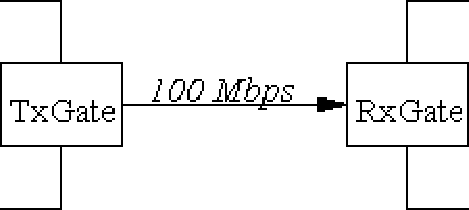
\includegraphics[width=2.315in, height=1.015in]{figures/usmanFig9}
    \caption{Connection with a data rate}
    \label{fig:ch-simple-modules:conn-w-data-rate}
  \end{center}
\end{figure}

While a message is under transmission, other messages have to wait
until the transmission finishes. You can still use \fname{send()}
while the gate is busy, but the message's arrival will be delayed;
just like the gate had an internal queue for the messages waiting to
be transmitted.


The {\opp} class library provides you with functions to check
whether a certain output gate is transmitting or to learn when
it finishes transmission.


If the connection with a data rate is not the immediate one connected
to the simple module's output gate but the second
one in the route, you have to check the second gate's busy
condition\index{gate!busy condition}.


\textbf{Implementation of message sending}


Message sending is implemented in the following way: the arrival
time\index{arrival time} and the bit error\index{bit error} flag of a
message are calculated at once, when the \fname{send()} (or similar)
function is invoked. That is, if the message travels through several
links until it reaches its destination, it is \textit{not} scheduled
individually for each link, but rather, every calculation is done
once, within the \fname{send()} call. This implementation was chosen
because of its run-time efficiency.

In the actual implementation of queuing the messages at busy gates and
modeling the transmission delay, messages do not actually queue up in
gates; gates do not have internal queues. Instead, as the time when
each gate will finish transmission is known at the time of sending the
message, the arrival time\index{arrival time} of the message can be
calculated in advance. Then the message will be stored in the event
queue (FES)\index{FES} until the simulation time advances to its
arrival time and it is retrieved by its destination module.

%
% TBD add pseudocode
%


\textbf{Consequence}


The implementation has the following consequence. If you change the
delay (or the bit error rate, or the data rate) of a link\index{link
  delay} during simulation, the modeling of messages sent ``just
before'' the parameter change will not be accurate. Namely, if link
parameters change while a message is ``under way'' in the model, that
message will not be affected by the parameter change, although it
should. However, all subsequent messages will be modelled correctly.
Similar for data rate: if a data rate changes during the simulation,
the change will affect only the messages that are \textit{sent} after
the change.

If it is important to model gates and channels with changing
properties, you can go two ways:
\begin{itemize}
  \item{write sender module such that they schedule events for when the
    gate finishes its current transmission and send then;}
  \item{alternatively, you can implement channels with
    simple modules (``active channels'').}
\end{itemize}

\textbf{The approach of some other simulators}


Note that some simulators (e.g. OPNET) assign \textit{packet queues}
to input gates (ports), and messages sent are buffered at the
destination module (or the remote end of the link) until received by
the destination module. With that approach, events and messages are
separate entities, that is, a \textit{send} operation includes placing
the message in the packet queue \textit{and} scheduling an event which
will signal the arrival of the packet. In some implementations, also
output gates have packet queues where packets wait until the channel
becomes free (available for transmission).

{\opp} gates\index{gate} don't have associated queues. The place
where the sent but not yet received messages are buffered is the
\textit{FES}\index{FES}.  {\opp}'s approach is potentially faster
than the above mentioned solution because it doesn't have the
enqueue/dequeue overhead and also spares an event creation. The
drawback is, as mentioned above, that changes to channel parameters do
not take effect immediately.





\section{Coding conventions}

Here's a bunch of advice on how to write {\opp} models. Some
of them are ``rules of thumb'', saying if you program like that,
you're likely to have less trouble; other conventions are aimed
at making the models produced by the {\opp} community more consistent.


Conventions for writing simple\index{module!simple} modules:
\index{module!conventions}
\begin{enumerate}
\item{Put the NED description, the C++ class declaration and the
    implementation into three separate files. Do not put two or more
    modules' code into the same file unless they are build upon one
    another - don't be afraid of small files! Thus, for a
    simple module called Foobar, you should have
    Foobar.ned, Foobar.h and Foobar.cc. This reduces coupling of
    module sources and makes your code more reusable.}
\item{Adopt a good coding style. Some hints: Choose your favourite
    indentation style and keep to that consistently. I recommend
    four-space indents and the brace placement style in which the
    {\opp} sources are written. Write only one statement per line.
    Avoid putting comments at the end of the line - place them
    \textit{above} the code on a separate line instead! Use blank
    lines to break the code into not-very-long logical blocks, and put
    a few-word comment above each block what that block does. Leave at
    least two blank lines between two (member) functions. The purpose
    of all that is that the structure of your code be obvious at the
    first glance!}
\item{Identifiers: Begin module type names with a capital letter, and
    capitalize the beginning of each word, like in \ttt{TokenRingMAC}.  Do
    not use underscore `\_' in module names. Use the C++-style naming
    on member functions: beginning of each word is capitalized (except
    for the first one) and no underscores: sendUnnumberedFrame().}
\item{Make the functions virtual. Maybe someone who reuses your code
    will need a different behavior than what you thought of.}
\item{Use inheritance\index{inheritance} if you're writing a very complex
    simple module: create a basic
    simple module class and build upon it
    deriving new module classes. This will make your code more
    readable and easier to manage/reuse. Unfortunately, inheritance is
    not supported in NED so you actually have to make distinct NED
    descriptions for each simple module class.
    Even if you have an abstract classes, prepare a NED description
    for it: it is useful as a reference to others who might derive a
    different simple module class from your
    abstract class. Inheritance in NED\index{ned!inheritance} is
    planned in later releases of {\opp}.}
\item{Avoid global variables\index{global variables} (and what's the
    same, static class members).  They are not reset to their initial
    value (zero) when you run the simulation, stop it and rebuild the
    network. This can cause several problems when you use Cmdenv to
    execute several runs one after another, or in Tkenv when you
    rebuild the network from the menu.}
\item{Query the values of parameters into state variables
    (--\texttt{>}class members) of the \textit{same} name at the top
    of the \fname{activity()} function.  If you know the value of a
    parameter is a random value (like uniform 0..10) or it can change
    during simulation, then to avoid having to look it up by name each
    time (like \ttt{d=par(''delay'')}) you may query its pointer into a
    \cclass[cPar]{cPar*} state variable with the same name prepended with
    `p' (like \ttt{pDelay=\&par(''delay'')}).}
  \item{Use \fname{ev.printf()} and \texttt{ev <}\texttt{<}... (see
    later) to print out information on what the module is doing. Doing
    so will pay out several times when it comes to debugging. Use a
    parameter and a state variable called debug. Surround your
    debugging output (\texttt{ev <}\texttt{<}... and
    \fname{ev.printf()} calls) with \texttt{if(debug)}.  You may
    introduce more specific debug switches (like debug\_queuing etc.)}
\end{enumerate}



\section{Some simulation techniques}

\subsection{Modeling computer networks}

The hierarchical module structure of {\opp} allows you to organize
the model around different levels:

Physical topology:
\begin{enumerate}
  \item{Top-level network}
  \item{Subnetwork (site)}
  \item{LAN}
  \item{node}
\end{enumerate}

Within a node:
\begin{enumerate}
  \item{OSI layers. The Data-Link, Network, Transport, Application layers
        are of greater importance.}
  \item{Applications/protocols within a layer.}
\end{enumerate}

The advantage of {\opp} over many existing simulators is that the
depth of the module nesting\index{module!nesting depth} is not
limited, and, what is in connection with the previous one, that a
simple module can be transformed into a
compound\index{module!compound} module by splitting the code into
several simple\index{module!simple} modules \textit{without affecting
  existing users} of the module and vice versa. The latter means that
the programmer of the model is not under pressure from possibly
incorrect early design decisions about what to implement with a single
module and what with a compound\index{module!compound} module.



\subsection{Modeling multiprocessor systems}

One can make use of flexible model topologies. It is straightforward
to create ring, mesh, butterfly, torus, hypercube, tree, fat tree and
other topologies with conditional loop
connections\index{connection!loop}.


Furthermore, general \textit{topology
  templates}\index{topology!templates} (e.g. mesh or hypercube) can be
created, where the types of the actual nodes are left as parameters.
The actual node types are substituted as parameter values for each
concrete simulation. Topology templates could be placed in a library
and imported from there if needed.





\subsection{Parameter tuning}

Tuning means finding the parameter values which produce optimal
operation of the system. In {\opp}, you can tune the model during
runtime. The code that monitors performance and changes parameter
values can be placed:
\begin{itemize}
\item{inside the model. In this case, the code does not necessarily
    form separate module(s); you can add the extra code to any already
    existing module.}
\item{outside the model of the actual system. If you choose this
    method, you will create new modules that monitor and control the
    model.}
\end{itemize}

{\opp} supports the model tuning\index{model!tuning} concept by
providing reference parameters. Parameters that influence the model
performance and need to be tuned will be declared at the highest layer
and taken by both the model and the monitor part.


An example of model tuning is how one can determine the critical
throughput of a communication network by changing the offered
load according to performance measures of the network (queuing
times etc.)





\subsection{Multiple experiments within one simulation run}

One might need to perform a large number of simulation runs where
the model parameters are not known in advance. This can be the
case when one wants to optimize a system and parameter tuning
cannot be used because
\begin{enumerate}
\item{for each experiment, he wants to start the model from a
    well-defined initial state, or}
\item{he wants to change the model topology from one simulation run to
    the other}
\end{enumerate}

In this case, the following solution be followed. The network would
consist of only one simple module that would
organize the simulation runs by creating, running and destroying the
actual models with each experiment. The simple
module's code would look like this:


\begin{Verbatim}[commandchars=\\\{\}]
\textit{SimulationManager::activity()}
\{
    determine parameters for the first run
    while(true)
    \{
        create the model (a compound module) with the current
          run parameters schedule
        wait( some time) // while the model runs
        delete future events that belong to the model
        get statistics out of the model
        destroy the model
        if (simulation is done)
            break
        calculate parameters for the next run
    \}
    write out results
\}
\end{Verbatim}


The solutions built into {\opp} (flexible module topologies, dynamic
creation of compound modules etc.) strongly
support this concept.





\subsection{Dynamic topology optimization}

Dynamic topology optimization\index{topology!dynamic optimization} is
the generalization of the ``parameter tuning'' and ``multiple
experiments within one simulation run'' concepts. If one wants to
simulate large systems, it is possible that one part of the model
needs its topology to be optimized (optimal number of servers, optimal
interconnection etc.) while other parts of the model have reached
their steady state and should not be bothered.


This can be achieved by modifying the previous scheme. Parts
of the model that do not need topology optimization can be created
once and left running for the whole duration of the simulation;
other parts are examined and their structure is modified from
time to time.



%%% Local Variables:
%%% mode: latex
%%% TeX-master: "usman"
%%% End:
